\documentclass[spanish]{beamer}
\usepackage[ansinew]{inputenc} % Acepta caracteres en castellano
\usepackage[spanish]{babel}    % silabea palabras castellanas
\usepackage{amsmath}
\usepackage{mathtools,cancel} % cancela con una flecha \cancelto{0}{XXXX}
\renewcommand{\CancelColor}{\color{red}} %change cancel color to red
\usepackage{amsfonts}
\usepackage{amssymb}
\usepackage{dsfont}
\usepackage{graphicx}
\usepackage{geometry}
\usetheme{Madrid}
\usecolortheme{beaver}
\usepackage{textpos}
% Logo  en el comienzo 
\addtobeamertemplate{frametitle}{}{%
\begin{textblock*}{100mm}(.85\textwidth,-1cm)
{\includegraphics[height=0.4in, keepaspectratio=true]{/Users/luisnunez/Dropbox/MisDocumentos/UIS/UISImagenInstitucional/UISLOGO.png}}
\end{textblock*}}

\begin{document}

\title{\textbf{Dos Problemas S�lidos} }
\author[L.A. N��ez]{\textbf{Luis A. N��ez}}  
\institute[UIS]{\textit{Escuela de F�sica, Facultad de Ciencias, } \\
\textit{Universidad Industrial de Santander, Santander, Colombia } \\
{\includegraphics[height=0.4in, keepaspectratio=true]{/Users/luisnunez/Dropbox/MisDocumentos/UIS/UISImagenInstitucional/UISLOGO.png}}
}
\date{\today}
\maketitle


\begin{frame}
\frametitle{Agenda}
  \tableofcontents
\end{frame}


%%%%% Diapo 1
\section{Moneda que rueda sin deslizar}
\subsection{Ligaduras}
\frame{
  \frametitle{Moneda que rueda sin deslizar: Ligaduras}
Un disco homog�neo (una moneda) de radio $a$ y masa $M$ rueda sin deslizar por una superficie plana. Escriba las ecuaciones de movimiento y encuentre una soluci�n en el caso en que la inclinaci�n del disco sea constante.
\begin{figure}[t]
	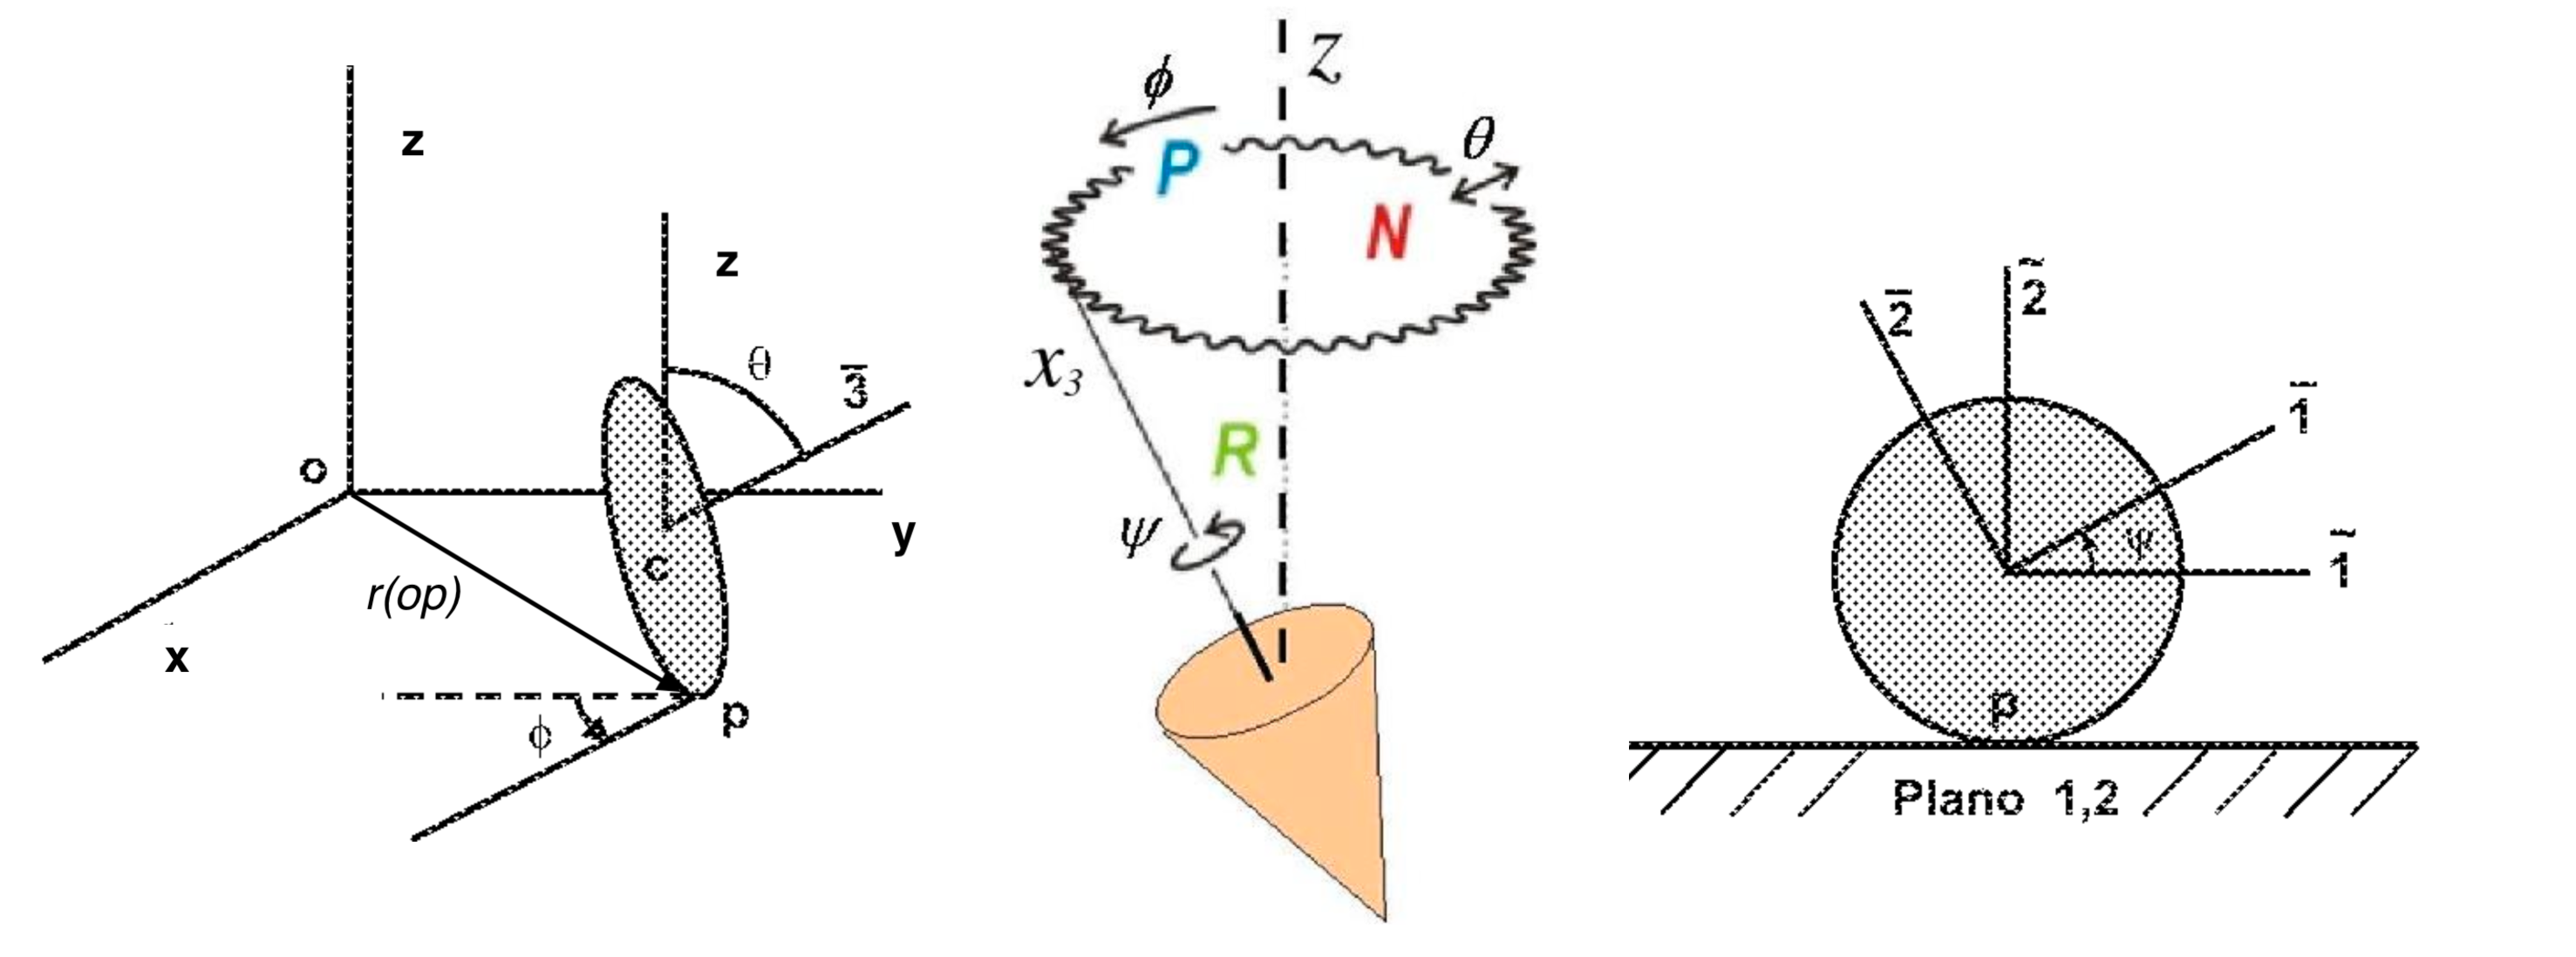
\includegraphics[width=2.8in]{Figuras/Moneda.pdf}
\end{figure}
   \begin{itemize}  
  	\item<1-> En principio tendremos seis grados de libertad $(x, y, z, \phi, \psi, \theta)$: tres de traslaci�n y tres �ngulos de Euler. 
	\item<3->  La ligadura de rodar sin deslizar implica que la velocidad del punto $p$, en contacto con la superficie, es instant�neamente cero.
	\item<4-> Esto es: $\vec{r}(op)=\vec{R}+\vec{r}(cp) \Rightarrow \dot{\vec{r}}(op)_{p}=0=\dot{\vec{R}}+  \vec{\Omega} \times \vec{r}(cp)$ 
    \end{itemize}
}
%%%%% Diapo 2
\subsection{El Lagrangeano}
\frame{
\frametitle{Moneda que rueda sin deslizar: Lagrangeano}
\begin{itemize}
	\item<1-> Por su parte, respecto al sistema centro de masa, $\tilde{S}$ tenemos $\vec{r}(cp) = -a {\bf x}_2$, y $\vec{\Omega} \times \vec{r}(cp) = 
	\left|
	\begin{array}{ccc} 
	{\bf x}_1 & {\bf x}_2 & {\bf x}_3 \\
	\Omega_1 & \Omega_2 & \Omega_3 \\
	0 & -a & 0
	\end{array}\right| = a(\Omega_3 \, {\bf x}_1 -\Omega_1\, {\bf x}_3) $
	\item<2-> Respecto al sistema centro de masa 
	$\Omega_1  = \dot{\phi} \operatorname{sen} \, \theta \operatorname{sen} \, \psi+\dot{\theta} \cos \psi $ \\
	$\Omega_2  = \dot{\phi} \operatorname{sen} \, \theta \cos \psi-\dot{\theta} \operatorname{sen} \, \psi \quad $  y 
	$\quad \Omega_3  = \dot{\psi}+\dot{\phi} \cos \theta$
	\item<2-> Proyectamos la ecuaci�n $0=\dot{\vec{R}}+  \vec{\Omega} \times \vec{r}(cp)$ al sistema $S$, (${\bf i}$, ${\bf j}$, ${\bf k}$) tendremos 
	$\dot{x} + a(\Omega_3 \, {\bf i} \cdot {\bf x}_1 -\Omega_1\, {\bf i} \cdot {\bf x}_3) = 0 $ \\
	$\dot{y} + a(\Omega_3 \, {\bf j} \cdot {\bf x}_1 -\Omega_1\, {\bf j} \cdot {\bf x}_3) = 0 $ \\
	$\dot{z} + a(\Omega_3 \, {\bf k} \cdot {\bf x}_1 -\Omega_1\, {\bf k} \cdot {\bf x}_3) = 0 $
\end{itemize} 
}
%%%%% Diapo 2
\section{Secci�n}
\frame{
\frametitle{T�tulo transparencia}
\begin{itemize}
	\item<1-> La energ�a cin�tica ser� $\left.T=\frac{1}{2} M\left(\dot{x}^2+\dot{y}^2+\dot{z}^2\right)+\frac{1}{2}\left[I_{1}(c)\left(\Omega_{1}\right)^2+I_{2}(c)\left(\Omega_{2}\right)^2+I_{3}(c) \Omega_{3}\right)^2\right]$.  
	\item<2-> 	$T=\frac{1}{2} M\left(\dot{x}^2+\dot{y}^2+\dot{z}^2\right)+\frac{1}{8} M a^2\left[\dot{\phi}^2 \operatorname{sen}^2 \theta+\dot{\theta}^2+2\left(\dot{\phi} \cos \theta^2+\dot{\psi}\right)^2\right]$
	\item<2-> Donde $I_{1}=I_{2}=M a^2 / 4$ y $I_{3}=M a^2 / 2$.
	\item<3-> Por su parte, la energ�a potencial $V = mga \operatorname{sen} \theta$
	\item<4-> El Lagrangeano $\mathcal{L} = T-V$, $\mathcal{L} = \frac{1}{2} M\left(\dot{x}^2+\dot{y}^2+\dot{z}^2\right)+\frac{1}{8} M a^2\left[\dot{\phi}^2 \operatorname{sen}^2 \theta+\dot{\theta}^2+2\left(\dot{\phi} \cos \theta^2+\dot{\psi}\right)^2\right] - mga \operatorname{sen} \theta$

\end{itemize}
}

  
\end{document}

%%%%% Diapo 2
\section{Secci�n}
\frame{
\frametitle{T�tulo transparencia}
\begin{itemize}  
	\item<1-> 
\end{itemize}
}
	\item<2->Las tres primeras components con las coordenadas cartesianas del centro $c$ y las siguientes los �ngulos de Euler. Adem�s $\vec{r}(c p)=-a {\bf k}}$.

	\begin{figure}[t]
		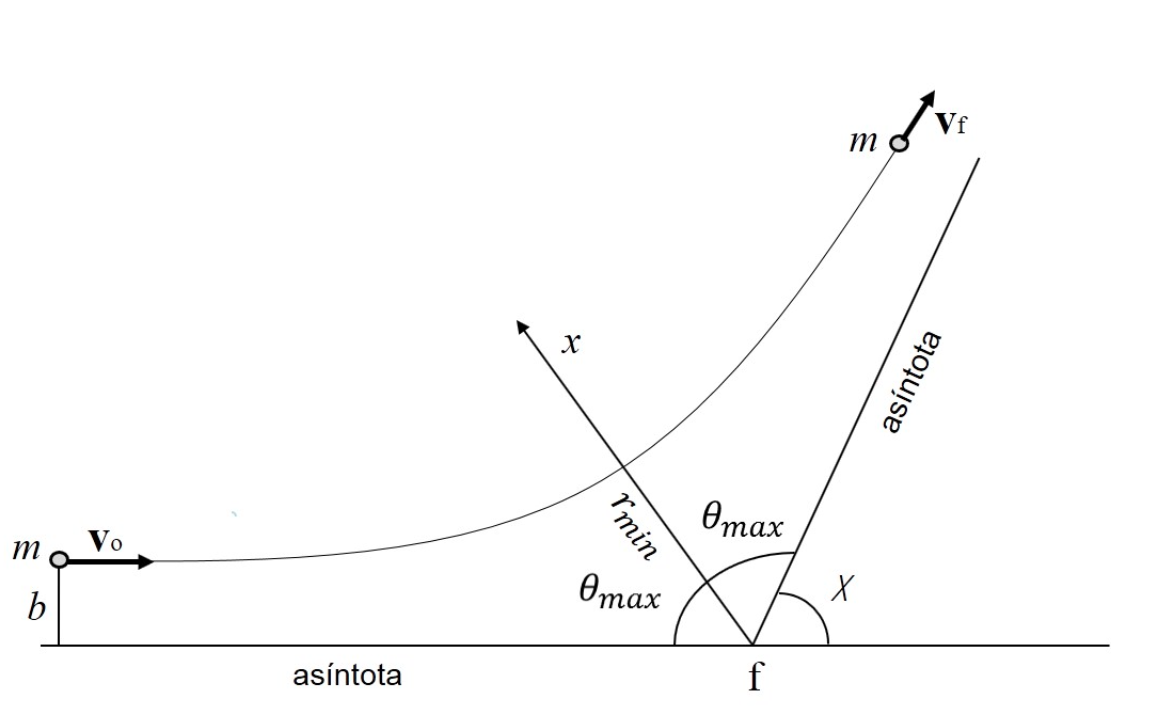
\includegraphics[width=1.8in]{Figuras/Dispersion.png}
   	\end{figure}
	
